% Hlavicka pro protokoly z fyzikalniho praktika.
% Verze pro: LaTeX
% Verze hlavicky: 22. 2. 2007
% Autor: Ustav fyziky kondenzovanych latek
% Ke stazeni: www.physics.muni.cz/ufkl/Vyuka/
% Licence: volne k pouziti, nejlepe k vcasnemu odevzdani protokolu z Vaseho mereni.

\documentclass[a4paper,11pt]{article}

% Kodovani (cestiny) v dokumentu: utf-8
%\usepackage[cp1250]{inputenc}	% Omezena stredoevropska kodova stranka, pouze MSW.
\usepackage[utf8]{inputenc}	% Doporucujeme pouzivat UTF-8 (unicode).

%%% Nemente:
\usepackage[margin=2cm]{geometry}
\newtoks\jmenopraktika \newtoks\jmeno \newtoks\datum
\newtoks\obor \newtoks\skupina \newtoks\rocnik \newtoks\semestr
\newtoks\cisloulohy \newtoks\jmenoulohy
\newtoks\tlak \newtoks\teplota \newtoks\vlhkost
\usepackage{amsmath}
\usepackage{mathtools}
\usepackage{graphicx}
\usepackage{multirow}
\graphicspath{ {./images/} }
%%% Nemente - konec.


%%%%%%%%%%% Doplnte pozadovane polozky:

\jmenopraktika={Fyzikální praktikum 2}  % nahradte jmenem vaseho predmetu
\jmeno={Artem Gorodilov}            % nahradte jmenem mericiho
\datum={16. ~listopadu  2023}        % nahradte datem mereni ulohy
\obor={Astrofyzika}                     % nahradte zkratkou vami studovaneho oboru
\skupina={Čt 8:00}            % nahradte dobou vyuky vasi seminarni skupiny
\rocnik={II}                  % nahradte rocnikem, ve kterem studujete
\semestr={I}                 % nahradte semestrem, ve kterem studujete

\cisloulohy={9}               % nahradte cislem merene ulohy
\jmenoulohy={Měření závislosti indexu lomu skla a vlnové délce metodou minimální derivace} % nahradte jmenem merene ulohy

\tlak={974}                   % nahradte tlakem pri mereni (v hPa)
\teplota={22.3}               % nahradte teplotou pri mereni (ve stupnich Celsia)
\vlhkost={51}               % nahradte vlhkosti vzduchu pri mereni (v %)

%%%%%%%%%%% Konec pozadovanych polozek.


%%%%%%%%%%% Uzitecne balicky:
\usepackage[czech]{babel}
\usepackage{graphicx}
\usepackage{amsmath}
\usepackage{xspace}
\usepackage{url}
\usepackage{indentfirst}
\usepackage{listings}
\usepackage{subcaption}
\usepackage{caption}
\usepackage{tabularx}
\usepackage[labelformat=parens,labelsep=quad,skip=3pt]{caption}

%%%%%% Zamezeni parchantu:
\widowpenalty 10000 \clubpenalty 10000 \displaywidowpenalty 10000
%%%%%% Parametry pro moznost vsazeni vetsiho poctu obrazku na stranku
\setcounter{topnumber}{3}	  % max. pocet floatu nahore (specifikace t)
\setcounter{bottomnumber}{3}	  % max. pocet floatu dole (specifikace b)
\setcounter{totalnumber}{6}	  % max. pocet floatu na strance celkem
\renewcommand\topfraction{0.9}	  % max podil stranky pro floaty nahore
\renewcommand\bottomfraction{0.9} % max podil stranky pro floaty dole
\renewcommand\textfraction{0.1}	  % min podil stranky, ktery musi obsahovat text
\intextsep=8mm \textfloatsep=8mm  %\intextsep pro ulozeni [h] floatu a \textfloatsep pro [b] or [t]

% Tecky za cisly sekci:
\renewcommand{\thesection}{\arabic{section}.}
\renewcommand{\thesubsection}{\thesection\arabic{subsection}.}
% Jednopismenna mezera mezi cislem a nazvem kapitoly:
\makeatletter \def\@seccntformat#1{\csname the#1\endcsname\hspace{1ex}} \makeatother

\begin{document}

\thispagestyle{empty}

{
\begin{center}
\sf 
{\Large Ústav fyzikální elektroniky PřF MU} \\
\bigskip
{\huge \bfseries FYZIKÁLNÍ PRAKTIKUM} \\
\bigskip
{\Large \the\jmenopraktika}
\end{center}

\bigskip

\sf
\noindent
\setlength{\arrayrulewidth}{1pt}
\begin{tabular*}{\textwidth}{@{\extracolsep{\fill}} l l}
\large {\bfseries Zpracoval:}  \the\jmeno & \large  {\bfseries Naměřeno:} \the\datum\\[2mm]
\large  {\bfseries Obor:} \the\obor  \hspace{40mm}  {\bfseries Skupina:} \the\skupina %
%{\bfseries Ročník:} \the\rocnik \hspace{5mm} {\bfseries Semestr:} \the\semestr  
&\large {\bfseries Testováno:}\\
\\
\hline
\end{tabular*}
}

\bigskip

{
\sf
\noindent \begin{tabular}{p{3cm} p{0.6\textwidth}}
\Large  Úloha č. {\bfseries \the\cisloulohy:} \par
\smallskip
$T=\the\teplota$~$^\circ$C \par
$p=\the\tlak$~hPa \par
$\varphi=\the\vlhkost$~\%
&\Large \bfseries \the\jmenoulohy  \\[2mm]
\end{tabular}
}

\vskip1cm
    \begin{minipage}[t]{0.5\textwidth} 
    \section{Zadání}
        Změřit úhel lomu optického hranolu N-SF11
        \par Pro určité vlnové délky zjistit derivace a indexy lomu. 
        \par Určit Abbeovo číslo.
    \section{Teorie}
        \subsection{Index lomu}
            Pro určení indexu lomu optického hranolu použijeme metodu minimální derivace. K tomu je třeba určit úhel lomu hranolu, což je úhel mezi dvěma stranami hranolu, jimiž světelný paprsek vstupuje a vychází. Tento úhel lze určit z úhlu, který svírají paprsky kolmé na každou stranu hranolu, viz obrázek (\ref{fig:lom}). Úhel lomu $\omega$ se vypočítá podle následujícího vzorce:
            \begin{equation}
                \omega = 180^o - (\psi_1 - \psi_2)
            \end{equation}
            kde $\omega$ je úhel lomu a $\psi_1$ a $\psi_2$ jsou kolmý úhly dopadu na hranolu.
            \vspace{10pt}
            \par 
            \centering
            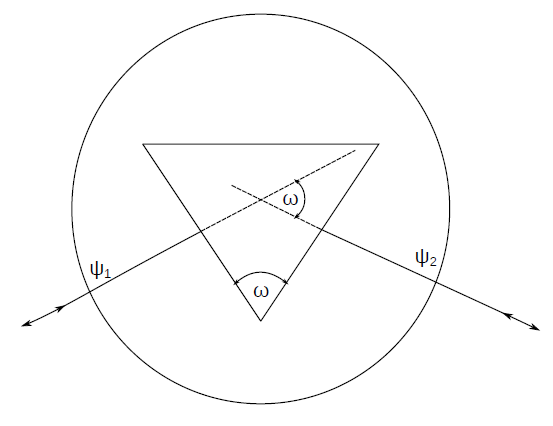
\includegraphics[scale=0.4]{lom}
            \captionsetup{justification=centering, font=footnotesize}
            \captionof{figure}{Měření úhlu lomu hranolu.}
            \label{fig:lom}
            \vspace{10pt}
            \raggedright
    \end{minipage}
    \hspace{10pt}
    \begin{minipage}[t]{0.5\textwidth} 
        \subsection{Úhel minimální derivace a Abbeovo číslo}
            Úhel minimální derivace $\delta_m$ představuje minimální úhel mezi světelným paprskem vstupujícím do hranolu $\varphi_1$ a vystupujícím z něj $\varphi_2$ viz obrázek (\ref{fig:der}). Pro jeho zjištění použijeme následující vzorec:
            \begin{equation}
                \delta_m = \frac{\varphi_1 - \varphi_2}{2} ~~,~~m~je~\lambda_m=1,2,3...
            \end{equation}
            kde $\delta_m$ je minimální derivace a $\varphi_1$ a $\varphi_2$ jsou úhly dopadu světla změřené goniometrem. 
            \par Je důležité si uvědomit, že úhel minimální derivace bude pro různé vlnové délky $\lambda_m$ různý. Proto budeme provádět měření pro určité vlnové délky odpovídající spektrálním čarám rtuťové výbojky. 
            \vspace{10pt}
            \par 
            \centering
            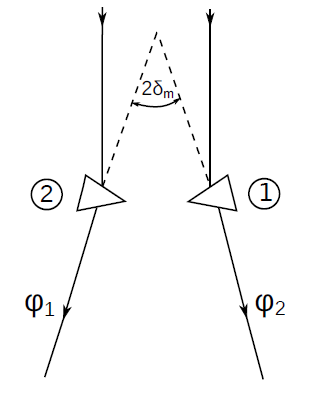
\includegraphics[scale=0.4]{der}
            \captionsetup{justification=centering, font=footnotesize}
            \captionof{figure}{Měření minimálního úhlu derivace $\delta_m$ od rozdílu úhlů $\varphi_1$ a $\varphi_2$, při kterém pozorujeme paprsky opouštějící hranol při vstupu první, resp. druhou lomenou stěnou (poloha hranolu). 1 a 2).}
            \label{fig:der}
            \vspace{10pt}
            \raggedright
            \par Nyní můžeme vypočítat index lomu $n$ materiálu pomocí vzorce:
            \begin{equation}
                n = \frac{sin\left(\frac{\delta_m + \omega}{2}\right)}{sin\left(\frac{\omega}{2}\right)}
            \end{equation}
    \end{minipage}
\newpage
    \begin{minipage}[t]{0.5\textwidth}
            Index lomu závisí na vlnové délce v důsledku disperze světla. K disperzi dochází v důsledku závislosti rychlosti šíření záření v prostředí na frekvenci záření. Tento jev lze popsat Cauchyho vztahem:
            \begin{equation}
                n(\lambda) = A + \frac{B}{\lambda^2}
            \end{equation}
            Z toho lze vypočítat Abbeovo číslo $\nu_d$, parametr popisující optické systémy. Abbeho číslo se odvozuje z indexů lomu pro Fraunhoferovy čáry: Žlutá $\lambda_d$ = 587.6 [nm], modrá $\lambda_F$ = 486.1 [nm] a červená $\lambda_C$ = 656.3 [nm] a lze ho vyjádřit následujícím vztahem:
            \begin{equation}
                \nu_d = \frac{n_d - 1}{n_F - n_C}
            \end{equation}
            kde $n_d$, $n_F$ a $n_C$ je indexy lomu pro vlnové délky $\lambda_d$, $\lambda_F$ a $\lambda_C$ resp. 
    \section{Měření}  
        \subsection{Index lomu}
            Na základě měření jsme změřili hodnoty kolmých úhlů dopadu $\psi_1$ a $\psi_2$, viz tabulku (1), a stejné úhly, ale pro tři jiné polohy hranolu na goniometru (třikrát jsme hranol mírně otočili ve směru hodinových ručiček), viz tabulku (2). Hodnoty úhlů lomu $\omega$ byly vypočteny podle vzorce (1).
            \vspace{10pt}
            \par \centering
            \begin{tabular}{|c|c|c|c|}
                    \hline
                    $\psi_1$ [$^o$] & $\psi_2$ [$^o$] & $\omega$ [$^o$] \\
                    \hline
                    260.8836(3) & 140.8831(3) & 59.9994(4) \\
                    \hline
                    260.8825(3) & 140.8825(3) & 60.0000(4) \\
                    \hline
                    260.8831(3) & 140.8842(3) & 60.0011(4) \\
                    \hline
                \end{tabular}
                \captionsetup{justification=centering, font=footnotesize}
                \captionof{table}{Naměřené hodnoty kolmých úhlů dopadu $\psi_1$ a $\psi_2$ a vypočtené úhly lomu $\omega$.}
                \raggedright
            \vspace{5pt}
            \par \centering
            \begin{tabular}{|c|c|c|c|}
                    \hline
                    $n$ & $\psi_1$ [$^o$] & $\psi_2$ [$^o$] & $\omega$ [$^o$] \\
                    \hline
                    1 & 283.4581(3) & 163.4586(3) & 60.0006(4) \\
                    \hline
                    2 & 278.5972(3) & 158.5989(3) & 60.0017(4) \\
                    \hline
                    3 & 272.9300(3) & 152.9289(3) & 59.9989(4) \\
                    \hline
                \end{tabular}
                \captionsetup{justification=centering, font=footnotesize}
                \captionof{table}{Naměřené hodnoty kolmých úhlů dopadu $\psi_1$ a $\psi_2$ a vypočtené úhly lomu $\omega$ pro různé úhly natočení hranolu na goniometru $n$.}
                \vspace{20pt}
                \raggedright
                \par Odtud můžeme zjistit hodnoty úhlu lomu $\omega$: 
                \begin{center}
                    $\omega$ = 60.000(1) 
                \end{center}
            \subsection{Úhel minimální derivace a Abbeovo číslo}
                Poté jsme změřili úhly dopadu $\varphi_1$ a $\varphi_2$ pro situaci znázorněnou na obrázku (\ref{fig:der}) pro různé vlnové délky $\lambda_m$ odpovídající různým barvám, viz tabulka (3). 
    \end{minipage}
    \hspace{10pt}
    \begin{minipage}[t]{0.5\textwidth}
                Poté jsme vypočítali úhel minimální derivace a index lomu hranolu pomocí vzorců (2) a (3), viz tabulka (4). 
                \vspace{10pt}
                \par \centering
                \begin{tabular}{|c|c|c|c|}
                    \hline
                    $Barvá$ & $\lambda$ [nm] & $\varphi_1$ [$^o$] & $\varphi_2$ [$^o$] \\
                    \hline
                    Červená & 623.4 & 275.9372(3) & 144.3614(4) \\
                    \hline
                    Žlutá & 576.9 & 276.6625(3) & 143.6414(4) \\
                    \hline
                    Zelená & 546.1 & 277.4144(3) & 142.8972(4) \\
                    \hline
                    Modrozelená & 491.6 & 279.1150(3) & 141.1753(4) \\
                    \hline
                    Modrá & 435.8 & 281.8831(3) & 138.3747(4) \\
                    \hline
                    Fialová & 404.6 & 284.3161(3) & 135.9431(4) \\
                    \hline
                \end{tabular}
                \captionsetup{justification=centering, font=footnotesize}
                \captionof{table}{Naměřené hodnoty kolmých úhlů dopadu $\varphi_1$ a $\varphi_2$ pro různé vlnové délky $\lambda_m$.}
                \vspace{5pt}
                \raggedright
                \par \centering
                \begin{tabular}{|c|c|c|c|}
                    \hline
                    $Barvá$ & $\lambda$ [nm] & $\sigma_m$ [$^o$] & $n$ \\
                    \hline
                    Červená & 623.4 & 65.7879(2) & 1.78032(2)\\
                    \hline
                    Žlutá & 576.9 & 66.5106(2) & 1.78604(2)\\
                    \hline
                    Zelená & 546.1 & 67.2586(2) & 1.79187(2)\\
                    \hline
                    Modrozelená & 491.6 & 68.9699(2) & 1.80494(2)\\
                    \hline
                    Modrá & 435.8 & 71.7542(2) & 1.82534(2)\\
                    \hline
                    Fialová & 404.6 & 74.1865(2) & 1.84227(2)\\
                    \hline
                \end{tabular}
                \captionsetup{justification=centering, font=footnotesize}
                \captionof{table}{Vypočtené úhly minimální derivace $\sigma_m$ a indexy lomu hranolu $n$ pro různé vlnové délky $\lambda_m$.}
                \vspace{10pt}
                \raggedright
                \par Vykreslíme závislost indexu lomu $n$ na vlnové délce $\lambda_m$ a sestrojíme fit podle vzorce (4). 
                \vspace{10pt}
                \par 
                \centering
                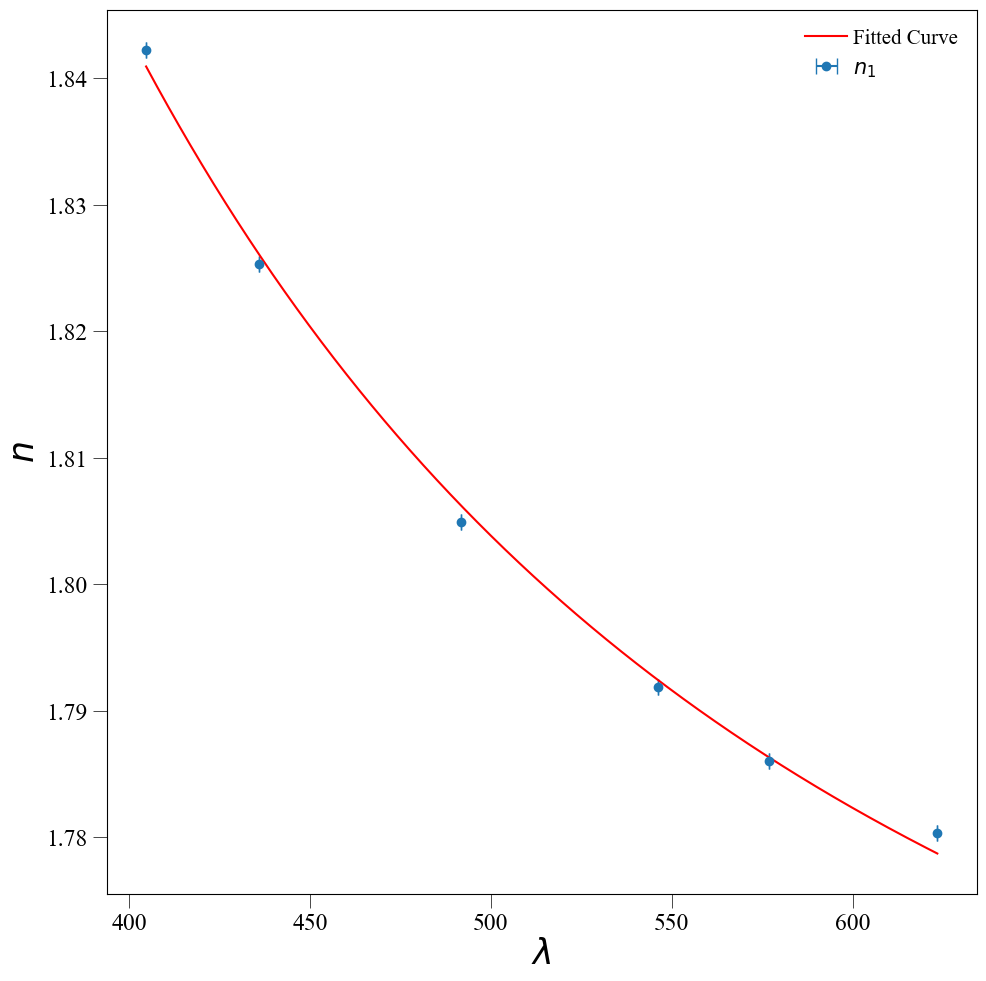
\includegraphics[scale=0.3]{index}
                \captionsetup{justification=centering, font=footnotesize}
                \captionof{figure}{Závislost indexu lomu $n$ na vlnové délce $\lambda_m$.}
                \label{fig:index}
                \vspace{10pt}
                \raggedright
                \par Proto byly získány následující hodnoty konstant $A$ a $B$:
                \begin{center}
                    $A$ = 1.73(2)
                    \vspace{5pt}
                    \par $B$ = 1.76(4) $\times$ 10$^4$
                \end{center}
    \end{minipage}
    \newpage
    \begin{minipage}[t]{0.5\textwidth} 
                Dále podle vzorce (4) zjistíme indexy lomu hranolů pro Fraunhoferovy čáry $n_d$, $n_F$ a $n_C$ a poté podle vzorce (5) zjistíme Abbeho číslo $\nu_d$:
                \begin{center}
                    $n_d$ = 1.784(2)
                    \vspace{5pt}
                    \par $n_F$ = 1.808(2)
                    \vspace{5pt}
                    \par $n_C$ = 1.774(2)
                    \vspace{5pt}
                    \par $\nu_d$ = 23.5(5)
                \end{center}
                K výpočtu veličin a jejich nejistot byla použita knihovna Uncertinties pro Python: \href{pypi.org/project/uncertainties}. Kód je přiložen k protokolu. 
        \section{Závěr}
            \subsection{Index lomu}
                Získali jsme hodnotu úhlu lomu $\omega$ = 60.000(1). S přihlédnutím k chybě hodnoty je velmi přesná. 
            \subsection{Úhel minimální derivace a Abbeovo číslo}
                Po výpočtech byly získány následující hodnoty indexů lomu pro Fraunhoferovy čáry: $n_d$ = 1.784(2), $n_F$ = 1.808(2) a $n_C$ = 1.774(2).
                \par Rovněž byla získána následující hodnota Abbeovo čísla: $\nu_d$ = 23.5(5), která odpovídá tabulkové hodnotě $\nu_d$ = 25.68 uvedené na stránce: \href{schott.com/shop/advanced-optics/en/Optical-Glass/N-SF11/c/glass-N-SF11} 
    \end{minipage}
\newpage
    \par K výpočtu chyb byl použit následující kód: 
    \begin{lstlisting}[language=Python, basicstyle=\tiny, breaklines=true]
        #Importing the libraries

        import matplotlib.pyplot as plt
        import numpy as np
        import pandas as pd
        from scipy import stats
        from scipy.optimize import curve_fit
        from uncertainties import *
        from uncertainties.umath import *

        #Reading data

        lom = pd.read_excel('lom.xlsx')
        waves = pd.read_excel('waves.xlsx')

        # Constants and values

        phi_1_1 = [283 , 27 , 29]
        phi_2_1 = [163 , 27 , 31]
        
        phi_1_2	= [278 , 35 , 50]
        phi_2_2 = [158 , 35 , 56]
        
        phi_1_3	= [272 , 55 , 48]
        phi_2_3 = [152 , 55 , 44]
        
        lambda_m = [623.4, 576.9, 546.1, 491.6, 435.8, 404.6]
        lambda_frau = np.array([656.3, 486.1, 587.6])
        
        radians = np.pi/180
        degrees = 180/np.pi

        def dms_to_decimal(degrees, minutes, seconds):
            decimal_degrees = degrees + (minutes / 60) + (seconds / 3600)
            return decimal_degrees

        # Calculation 

        lom['phi_1_decimal'] = dms_to_decimal(lom['phi_1_deg'], lom['phi_1_min'], lom['phi_1_sec'])
        lom['phi_2_decimal'] = dms_to_decimal(lom['phi_2_deg'], lom['phi_2_min'], lom['phi_2_sec'])
        
        waves['phi_1_decimal'] = dms_to_decimal(waves['phi_1_deg'], waves['phi_1_min'], waves['phi_1_sec'])
        waves['phi_2_decimal'] = dms_to_decimal(waves['phi_2_deg'], waves['phi_2_min'], waves['phi_2_sec'])
        waves['phi_2_2_decimal'] = dms_to_decimal(waves['phi_2_2_deg'], waves['phi_2_2_min'], waves['phi_2_2_sec'])
        
        phi_1_1_decimal = ufloat(dms_to_decimal(phi_1_1[0], phi_1_1[1], phi_1_1[2]), 0.000277778)
        phi_2_1_decimal = ufloat(dms_to_decimal(phi_2_1[0], phi_2_1[1], phi_2_1[2]), 0.000277778)
        
        # print('phi_1_1_decimal = ', phi_1_1_decimal)
        # print('phi_2_1_decimal = ', phi_2_1_decimal)
        
        phi_1_2_decimal = ufloat(dms_to_decimal(phi_1_2[0], phi_1_2[1], phi_1_2[2]), 0.000277778)
        phi_2_2_decimal = ufloat(dms_to_decimal(phi_2_2[0], phi_2_2[1], phi_2_2[2]), 0.000277778)
        
        # print('phi_1_2_decimal = ', phi_1_2_decimal)
        # print('phi_2_2_decimal = ', phi_2_2_decimal)
        
        phi_1_3_decimal = ufloat(dms_to_decimal(phi_1_3[0], phi_1_3[1], phi_1_3[2]), 0.000277778)
        phi_2_3_decimal = ufloat(dms_to_decimal(phi_2_3[0], phi_2_3[1], phi_2_3[2]), 0.000277778)
        
        # print('phi_1_3_decimal = ', phi_1_3_decimal)
        # print('phi_2_3_decimal = ', phi_2_3_decimal)
        
        lom_phi_1_list =[]
        lom_phi_2_list =[]
        for ii,ID in enumerate(lom['phi_1_decimal']):
            lom_phi_1_list.append(ufloat(lom['phi_1_decimal'][ii], 0.000277778))
            lom_phi_2_list.append(ufloat(lom['phi_2_decimal'][ii], 0.000277778))
        lom['phi_1_comb'] = lom_phi_1_list
        lom['phi_2_comb'] = lom_phi_2_list
        
        waves_phi_1_list =[]
        waves_phi_2_list =[]
        waves_phi_2_2_list =[]
        for ii,ID in enumerate(waves['phi_1_decimal']):
            waves_phi_1_list.append(ufloat(waves['phi_1_decimal'][ii], 0.000277778))
            waves_phi_2_list.append(ufloat(waves['phi_2_decimal'][ii], 0.000277778))
        waves['phi_1_comb'] = waves_phi_1_list
        waves['phi_2_comb'] = waves_phi_2_list
        
        lom['omega'] = 180 - (lom['phi_1_comb'] - lom['phi_2_comb'])
        
        omega_phi_1_1 = 180 - (phi_1_1_decimal - phi_2_1_decimal)
        omega_phi_1_2 = 180 - (phi_1_2_decimal - phi_2_2_decimal)
        omega_phi_1_3 = 180 - (phi_1_3_decimal - phi_2_3_decimal)
        
        # print('omega_phi_1_1 = ', omega_phi_1_1)
        # print('omega_phi_1_2 = ', omega_phi_1_2)
        # print('omega_phi_1_3 = ', omega_phi_1_3)

        omega_mean = ufloat(np.mean(np.array([np.mean(np.array(lom['omega'].apply(lambda x: x.nominal_value))), omega_phi_1_1.nominal_value, omega_phi_1_2.nominal_value, omega_phi_1_3.nominal_value])), np.sqrt(np.std(np.array([np.mean(np.array(lom['omega'].apply(lambda x: x.nominal_value))), omega_phi_1_1.nominal_value, omega_phi_1_2.nominal_value, omega_phi_1_3.nominal_value]))**2 + 0.000277778**2))
        print('omega_mean =', omega_mean)
        
        waves['sigma_1'] = (waves['phi_1_comb'] - waves['phi_2_comb']) / 2

        waves_n_1_list =[]
        for ii,ID in enumerate(waves['sigma_1']):
            waves_n_1_list.append(sin(radians * (waves['sigma_1'][ii] + omega_mean)/2)/sin(radians * omega_mean/2))
        waves['n_1'] = waves_n_1_list 
        
        # print(lom)
        # print(waves)

        # Define the polynomial function
        
        def polynomial_fit(lambda_values, A, B):
            return A + B / (lambda_values**2)
        
        # Use curve_fit to find the parameters A and B
        initial_guess = [1.5, 5000]  # Initial guess for parameters A and B
        params, covariance = curve_fit(polynomial_fit, lambda_m, waves['n_1'].apply(lambda x: x.nominal_value), p0=initial_guess)
        
        # Extract the optimized parameters
        A_optimized, B_optimized = params
        A_error, B_error = np.sqrt(np.diag(covariance))
        
        A_comb = ufloat(A_optimized, A_error)
        B_comb = ufloat(B_optimized, B_error)
        
        # Print the optimized parameters
        print('A =', A_comb)
        print('B =', B_comb)
        
        #Best-fit line
        
        lambda_val = np.linspace(404.6, 623.4, 1000)
        n_val = polynomial_fit(lambda_val, A_optimized, B_optimized)

        n_frau = polynomial_fit(lambda_frau, A_comb, B_comb)
        print('n_frau = ', n_frau)
        
        nu = (n_frau[2] - 1)/(n_frau[1] - n_frau[0])
        print('nu = ', nu)
    \end{lstlisting} 
\end{document}